\documentclass[12pt,a4paper,titlepage]{article}

\usepackage{IEEEtrantools} % For IEEE style bibliography

% Allow embedded images
\usepackage{graphicx}
\usepackage{float}

\usepackage[nottoc,notlof,notlot,numbib,section]{tocbibind} % Fix table of contents

\usepackage{pdfpages} % Allow embedded PDF pages

\usepackage{blindtext} % Lorem ipsum generator

% Fix URLs
\usepackage{url}
\usepackage[pdfborder={0 0 0},breaklinks=true]{hyperref}
\usepackage{breakurl}
\urlstyle{same}  % don't use monospace font for urls

\title{Development of an Underwater Acoustic Communication System for Sensor Networks or Robotics Applications}
\author{
  Dhesant Nakka \\
  Electronic \& Computer Engineering \\
  20146587 \\
  \texttt{djnakka@connect.ust.hk}
  \and
  Elvin Ruslim \\
  Electronic \& Computer Engineering \\
  20143585 \\
  \texttt{eruslim@connect.ust.hk}
  \and
  Professor Kam Tim Woo \\
  Electronic \& Computer Engineering \\
  \texttt{eetim@ust.hk}
}

\begin{document}
\maketitle

\pagenumbering{roman}
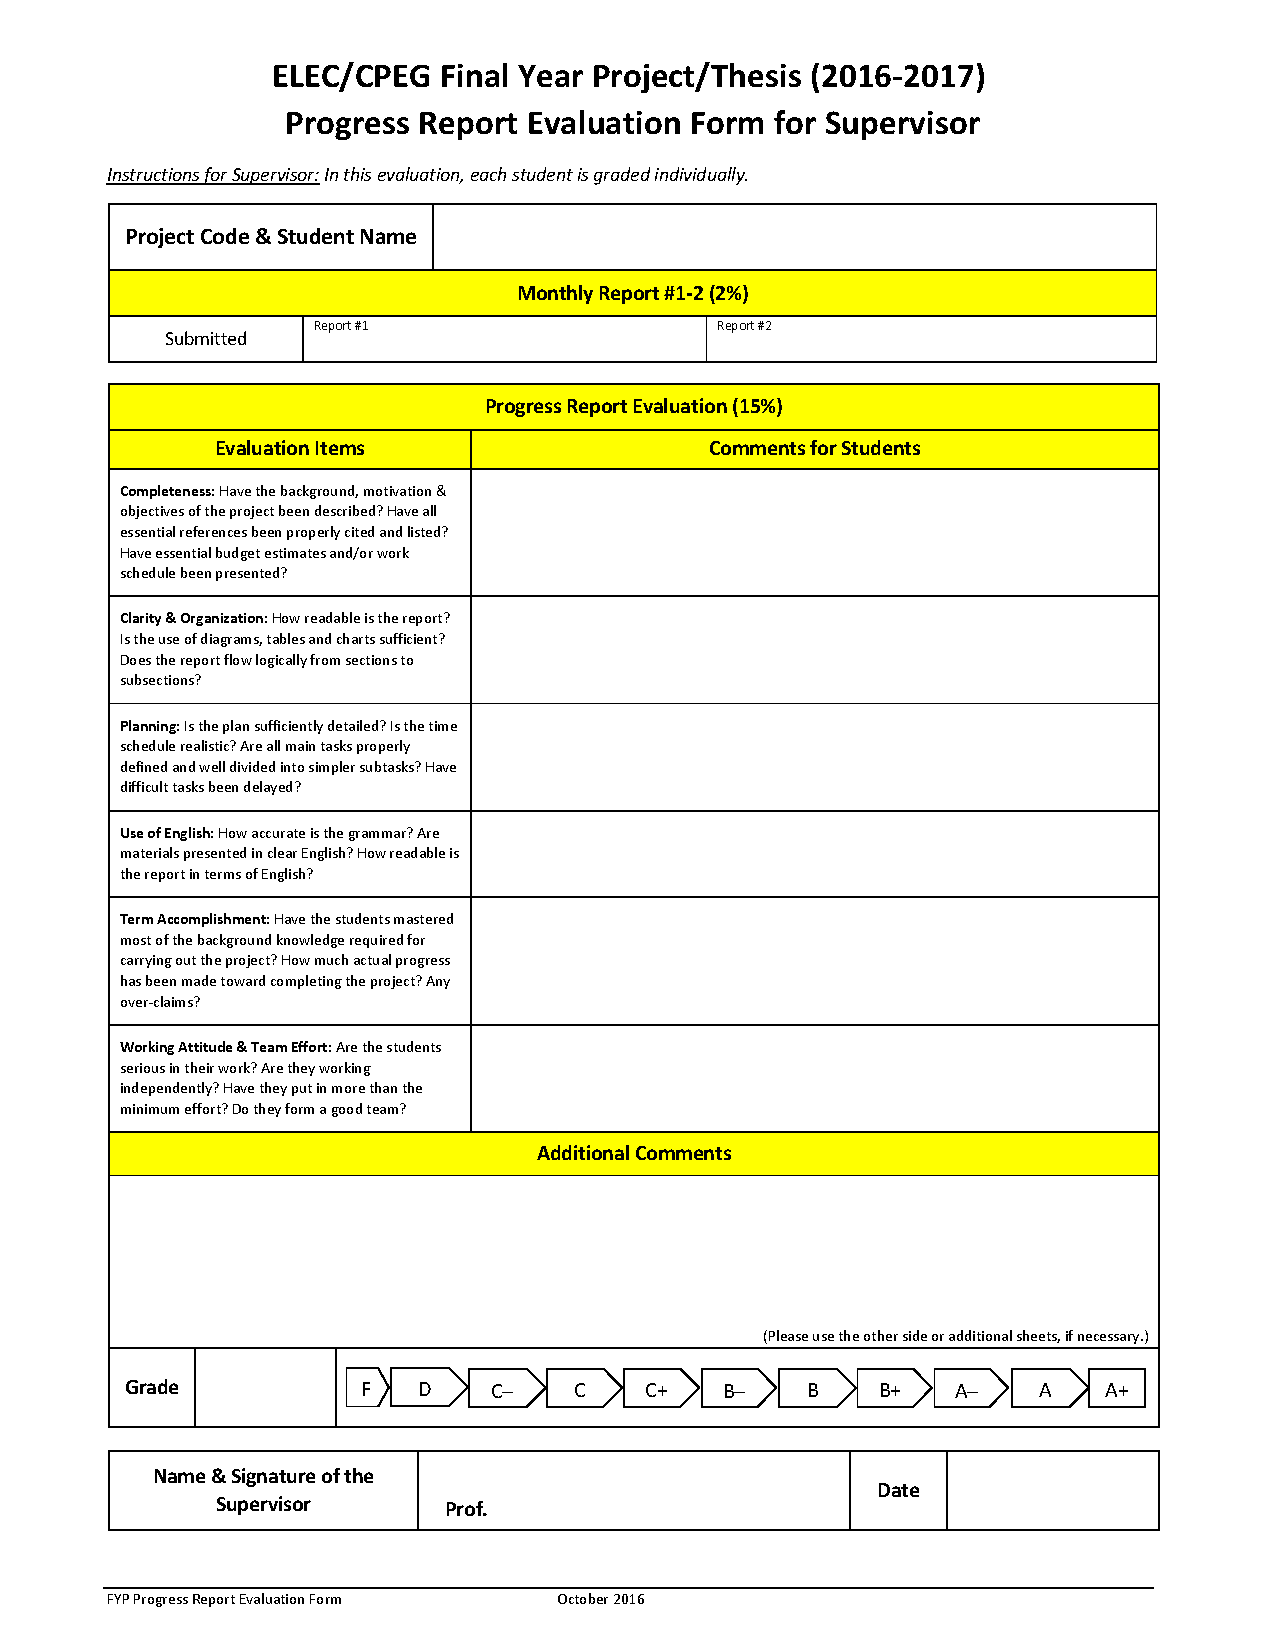
\includepdf{evaluation_form.pdf} % Add evaluation form for final PDF

\tableofcontents
%\newpage
\listoffigures
\listoftables

\newpage
\pagenumbering{arabic} % Restore page numbers

\section{Introduction}\label{sec:intro}
Over 70\% of the Earth’s surface is covered with water, and yet we have only explored less than 10\% of it. The main reason we have explored very little of the oceans because it is very hard for human beings to explore underwater. The traditional way to explore underwater environments is by diving, but diving is a very rigorous process, requiring extensive training, while having severe limitations on maximum depth, typically less than 40 meters for non-specialized applications \cite{padi}. The other way to explore is to use underwater robots. Underwater robots are much more capable than divers, with a typical depth rating of 3000 meters \cite{oe_rov}. However, because of their scarcity, they are typically custom built for a specific purpose, which makes them very expensive, costing millions of US dollars, making it very hard for anyone outside of a government organization, multinational company, or large research institute to use.

In recent years, this trend is starting to change, with the influx of cheap underwater robots starting to appear in the market \cite{trident,fathomone,ccrov}. This can be attributed by the adaptation of new technologies developed for different industries in underwater robotics, such as improvements in battery capacity and electric motors from electric vehicles, motion sensors from smart phones, or advanced materials from automotive and aerospace industries. However, one area that has been lacking is the development of an low-cost commercially viable underwater communication system, as there is little overlap with other industries where existing research can be leveraged. Because of this, these new robots are tethered to a remote operator on shore, severely reducing the range and effectiveness of these machines.

The aim of this project is to create a low-cost underwater wireless communication system using acoustic transceivers. Acoustic waves have favorable properties when underwater, where they can travel for thousands of miles, whereas more common wireless communication methods, such as Radio Frequency (RF) or Visible Light Communication (VLC) can only travel for a few hundred meters. Based on this observation, acoustic waves could be used to create a low-cost underwater communication system, greatly increasing the versatility of an underwater robotics platform, allowing for more flexible exploration opportunities.

\subsection{Report Outline}
\blindtext

\section{Literature Review}\label{sec:lit_review}
\Blindtext

\section{Project Overview}\label{sec:overview}
\subsection{Project Objectives}
\blindtext
\subsection{Individual Objectives}
\subsubsection{Dhesant Nakka}
\blindtext
\subsubsection{Elvin Ruslim}
\blindtext
\subsection{Project Description}
\blindtext

\subsection{Schedule}
\blindtext
\begin{figure}[H]
  \centering
  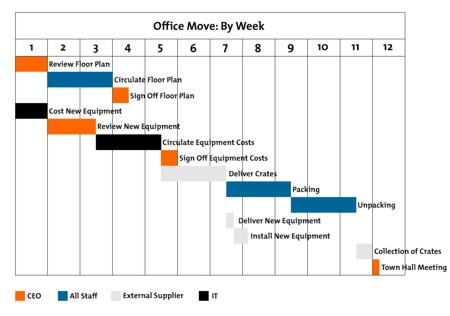
\includegraphics[width=\textwidth]{images/gantt_chart.jpg}
  \caption{Project Schedule Gantt Chart}
\end{figure}

\section{Project Details}\label{sec:details}
\blindtext
\subsection{Tasks}
\blindtext
\subsection{Expected Challenges}
\blindtext
\subsection{Budget}
\blindtext


\section{Proof of Concept}\label{sec:proof_concept}
\blindtext
\subsection{Design}
\blindtext
\subsection{Implementation}
\blindtext
\subsection{Testing}
\blindtext
\subsection{Results}
\blindtext

\section{Initial Prototype}\label{sec:intital_proto}
\blindtext
\subsection{Design}
\blindtext
\subsection{Implementation}
\blindtext
\subsection{Testing}
\blindtext
\subsection{Results}
\blindtext

\section{Summary}\label{sec:summary}
\Blindtext

\newpage
\bibliographystyle{IEEEtran}
\raggedright
\bibliography{progress_report.bib}

\end{document}
